\documentclass[12pt]{article}
\usepackage[T1]{fontenc}
\usepackage[margin=2cm]{geometry}

\usepackage{amssymb}
\usepackage{amsmath}
\usepackage{tcolorbox}
\usepackage{xcolor}
\usepackage{framed}
\usepackage{euscript}
\usepackage{float}

\usepackage{verbatim}
\usepackage{mathrsfs}
\usepackage{graphicx}
\usepackage{multicol}

\usepackage{bbm,txfonts}
\usepackage{float}


\usepackage{titletoc}
\usepackage{tikz}
\usepackage{xspace}

\usepackage{enumitem}

\newcommand{\answer}{\vspace*{4pt} \noindent{\bf Solution: }}

\newcommand{\bb}[1]{\mathbb{#1}}
\renewcommand{\v}[1]{\boldsymbol{#1}}
\newcommand{\m}[1]{\mathbf{#1}}
\renewcommand{\c}[1]{\mathcal{#1}}
\usepackage{upquote}


\renewcommand{\tilde}{\widetilde}
\newcommand{\halmos}{\vspace{3mm} \hfill \mbox{$\Box$}}

\newcommand{\Var}{\mathbb{V}\mathrm{ar}}
\newcommand{\var}{\Var}

\newcommand{\Cov}{\mathbb{C}\mathrm{ov}}
\newcommand{\cov}{\Cov}

\renewcommand{\epsilon}{\varepsilon}
\renewcommand{\rho}{\varrho}
\renewcommand{\log}{\ln}
\renewcommand{\hat}{\widehat}

\newcommand{\iid}{\text{iid }}


% Bernoulli distribution
\newcommand{\Ber}{{\sf Ber}}
\newcommand{\ber}{\Ber}

% Binomial distribution
\newcommand{\Bin}{{\sf Bin}}
\newcommand{\bin}{\Bin}

% Cauchy distribution
\newcommand{\Cauchy}{{\sf Cauchy}}

% Negative binomial distribution
\newcommand{\NegBin}{{\sf NegBin}}

% Multinomial distribution
\newcommand{\Mnom}{{\sf Mnom}}
\newcommand{\mnom}{\Mnom}

% Geometric distribution
\newcommand{\Geo}{{\sf Geom}}
\newcommand{\geo}{\Geo}
\newcommand{\Geom}{\Geo}
\newcommand{\geom}{\Geo}
\newcommand{\G}{\Geo}

% Hypergeometric distribution
\newcommand{\Hyp}{{\sf Hyp}}

% Poisson distribution
\newcommand{\Poi}{{\sf Poi}}
\newcommand{\poi}{\Poi}
\newcommand{\Po}{\Poi}
\newcommand{\po}{\Poi}

% Uniform distribution (continuous)
\newcommand{\U}{\EuScript{U}}

% Exponential distribution
\newcommand{\Ex}{{\sf Exp}}
\newcommand{\ex}{\Ex}

% Normal / Gaussian distribution
\newcommand{\Nor}{\EuScript{N}}
\newcommand{\nor}{\Nor}

% Pareto distribution
\newcommand{\Pareto}{{\sf Pareto}}
\newcommand{\pareto}{\Pareto}

% Negative hypergeometric distribution
\newcommand{\NegHyp}{{\sf NegHyp}}

% Student's t distribution
\newcommand{\Student}{{\sf t}}
\newcommand{\student}{\Student}

% Gamma distribution
\newcommand{\Gam}{{\sf Gamma}}
\newcommand{\gam}{\Gam}

% Discrete uniform distribution
\newcommand{\DU}{{\sf DU}}

% Generic distribution
\newcommand{\Dist}{{\sf Dist}}

\newcommand{\Em}{{\mathbb E}}  % expectation
\newcommand{\Pm}{{\mathbb P}}  % probability measure
\newcommand{\R}{{\mathbb R}}

\newcommand{\gvn}{\,|\,}  % conditional (given)

\newcommand{\e}{\mathrm{e}} %Euler's e

\newcommand{\ds}{\displaystyle}

\newcommand{\di}{\mathrm{d}}  % use for differential symbol


\newcommand{\approxsim}{\stackrel{\mathrm{approx.}}{\sim}}

\newcommand{\iidsim}{\stackrel{\mathrm{iid}}{\sim}}
\newcommand{\simiid}{\iidsim}
\newcommand{\simiidt}{{\:{\sim}_{\mathrm{iid}}\:}}

%% Correlation
\newcommand{\Corr}{\mathrm{Corr}}
\newcommand{\corr}{\Corr}


\usepackage{cprotect}
\RequirePackage[formats]{listings}\RequirePackage{textcomp}

\lstnewenvironment{Pout}{%
  \lstset{backgroundcolor=\color{outcol},
  aboveskip= -2pt,  
  xleftmargin = 4pt,
  xrightmargin = 4pt,
  frame=single,
  upquote,
  framerule=1pt,
  basicstyle=\footnotesize\ttfamily,
  columns=fixed}}{}

%DK: See http://latexcolor.com/
\definecolor{applegreen}{rgb}{0.55, 0.41, 0.0}
\definecolor{gray1}{rgb}{0.98, 0.98, 0.98}
\definecolor{black}{rgb}{0, 0, 0}
\definecolor{cream}{rgb}{1.0, 0.99, 0.82}
\definecolor{islamicgreen}{rgb}{0.0, 0.56, 0.0}
\definecolor{vlgray}{gray}{0.9}
\definecolor{lgray}{gray}{0.7}
\definecolor{outcol}{gray}{0.9}

\tcbuselibrary{listings,skins,breakable,theorems}

\newenvironment{PC}{%
\tcblisting{breakable,listing only,colback=cream, enhanced, sharpish
corners,  boxrule=1pt,after, listing options =
   {language=Python,
  basicstyle=\footnotesize\ttfamily,        % the size of the fonts that are used for the code
  numbers=none,                   % where to put the line-numbers
%  numberstyle=\tiny\color{blue},  % the style that is used for the line-numbers
  xleftmargin=-10pt,
  aboveskip=-4pt,
  belowskip=-6pt,
  columns=fixed,
  basewidth=5pt,                     %separation of letters
%  stepnumber=1,                % the step between two line-numbers. If it's 1, each line will be numbered
%  numbersep=7pt,                  % how far the line-numbers are from the code
  backgroundcolor=\color{cream},  % choose the background color. You must add \usepackage{color}
  showspaces=false,               % show spaces adding particular underscores
  showstringspaces=false,         % underline spaces within strings
  showtabs=false,                 % show tabs within strings adding particular underscores
  %frame=single,                   % adds a frame around the code
  %frame=shadowbox,
  %rulecolor=\color{black},        % if not set, the frame-color may be changed on line-breaks within not-black text (e.g. comments (green here))
  tabsize=2,                     % sets default tabsize to 2 spaces
 % captionpos=b,                  % sets the caption-position to bottom
  breaklines=true,                % sets automatic line breaking
  breakatwhitespace=false,        % sets if automatic breaks should only happen at whitespace
  %title=\lstname,                 % show the filename of files included with \lstinputlisting;
                                  % also try caption instead of title
  keywordstyle=\color{blue},      % keyword style
  upquote,     % very important to get right quote for cut/paste
  commentstyle=\color{islamicgreen},   % comment style
  stringstyle=\color{red},      % string literal style
 % escapeinside={\%*}{*)},         % if you want to add a comment within your code
  morekeywords={*,...}
  			 }
    		}
    	}
{\endtcblisting}







\usepackage{fvextra}
\DefineVerbatimEnvironment{Code}{Verbatim}{
    fontsize=\footnotesize, % Adjust font size
    breaklines=true,        % Enable line wrapping
    breakanywhere=true      % Allow breaking anywhere
}

\begin{document}
\begin{center}

{\Large  {\bf MACHINE LEARNING (COMP7703)}

Assignment - Semester 1, 2025.

\vspace{20pt}

{\large \textbf{Student Name:} Volter Entoma}
\vspace{10pt}

{\large \textbf{Student ID:} 44782711}

}
\end{center}

\vspace{20pt}

\textbf{1. Introduction}
\\
There are many different machine learning algorithms, and many metrics to evaluate them. In this assignment, we will focus on the K-Nearest Neighbour (K-NN) algorithm, Random Forest, and Deep Neural Networks, and the accuracy of each model. We will also looks at the different metrics to evaluate the performance of each model, and use these metrics to compare the suitability of each model for the given data.

\vspace{20pt}

\textbf{2. Aims}
\begin{itemize}
	\item To understand the K-Nearest Neighbour (K-NN) algorithm.
	\item To understand the accuracy of the K-NN classifier.
	\item To understand the effect of data imbalance on the accuracy of the K-NN classifier.
	\item To understand how to use cross-validation to improve the accuracy of the K-NN classifier.
\end{itemize}

\vspace{20pt}

\textbf{3. Data}
\\
The data used in this assignment is the \texttt{TTSWING} dataset, which is the provided dataset for this assignment. The dataset contains the 33 features, which are the 33 different measuremeents of table tennis swings. The dataset also contains the height of the player, which is the target variable. The dataset is a CSV file, and can be read into Python using the \texttt{pandas} library. The dataset is split into three categories: high, medium, and low.

\vspace{20pt}

\textbf{3.1 Data split}
\\
The data is split into three height categories: high, medium, and low. The data is split into 60\% training data, 20\% testing data, and 20\% validation data. The training data is used to train the each model, the testing data is used to test the accuracy of each model, and the validation data is used to compare the performance of the models. 

\vspace{20pt}

\textbf{3.2 Data imbalance}
\\
After splitting the data, there is an imbalance in the amount of training data assigned to each category in height. There are 17364 (29.73\%) data points in the high, 40800 (42.03\%) data points in the medium, and 27450 (28.23\%) in the low category. This is a significant imbalance; this imbalance is problematic because many machine learning algorithms tend to be biased toward the majority class. This can result in poor predictive performance for the minority classes, as the model may learn to ignore them in favor of achieving higher overall accuracy. In imbalanced datasets, accuracy becomes a misleading metric, since a model can achieve high accuracy by simply predicting the majority class most of the time, while failing to correctly classify minority class instances. This is especially concerning when the minority classes are of particular interest or importance.
\\
The data imbalanced is addressed by the use of Synthetic Minority Over-sampling Technique (SMOTE) to generate synthetic data points for the low category. The SMOTE algorithm generates synthetic data points by interpolating between existing data points in the low category. This is done by selecting a random data point from the low category, and then selecting a random data point from the k nearest neighbours of that data point. The synthetic data point is then generated by taking a weighted average of the two data points.
\\
After applying SMOTE, the training data is balanced, with 24552 data points in each category. All subsequent analysis is performed on the balanced training data. The testing and validation data is not balanced, and is used to test the accuracy of the models.
 
\vspace{20pt}

\textbf{3.3 Data standardization}


\textbf{4. Principle Component Analysis}

To investigate the effect of dimensionality reduction on the accuracy of the models, we will use Principle Component Analysis (PCA) to reduce the dimensionality of the data. PCA is a linear transformation that transforms the data into a new coordinate system, where the first coordinate is the direction of maximum variance, the second coordinate is the direction of maximum variance orthogonal to the first coordinate, and so on. 

% Insert figure of Scree plot here
\begin{figure}[h!]
\centering
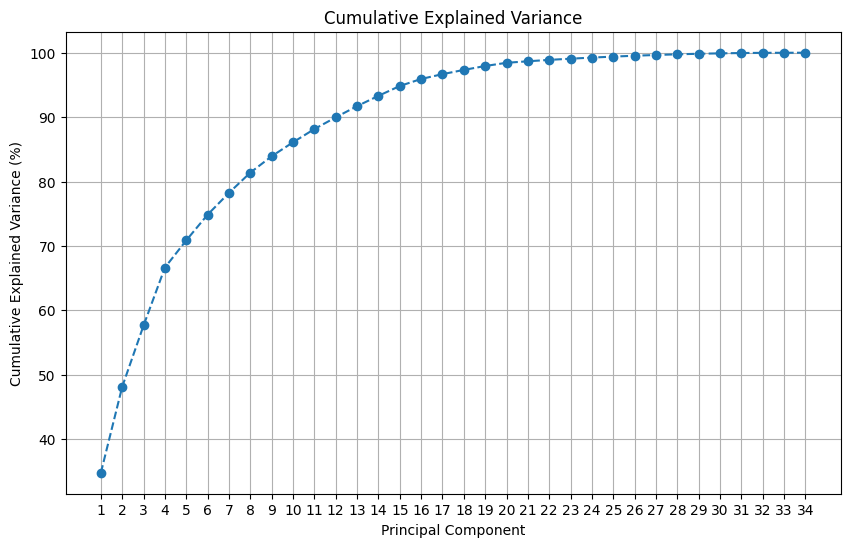
\includegraphics[width=0.8\textwidth]{figures/cum_var_scree.png}
\caption{Cumulative variance explained by each principal component.}
\label{fig:scree_plot}
\end{figure}

As shown in Figure \ref{fig:scree_plot}, approximately 95\% of the total variance is explained by the top 16 principal components. This allows us to reduce the dimensionality of our data from 33 dimensions to 16 dimensions while retaining the vast majority of the information content. This reduction offers several benefits:

\begin{itemize}
    \item Reduced computational complexity in subsequent modeling
    \item Mitigation of the curse of dimensionality
    \item Removal of potentially noisy or redundant features
    \item Improved model interpretability
\end{itemize}

The effectiveness of this dimensionality reduction will be evaluated by comparing model performance on both the original and PCA-reduced datasets.

\vspace{20pt}

\textbf{5. K-NN classifier}

The K-Nearest Neighbour (K-NN) algorithm is a simple and effective machine learning algorithm that can be used for both classification and regression tasks. The K-NN algorithm works by finding the k nearest neighbours of a data point, and then predicting the class of the data point based on the classes of the k nearest neighbours. The K-NN algorithm is a non-parametric algorithm, which means that it does not make any assumptions about the distribution of the data. This makes the K-NN algorithm very flexible, and it can be used for a wide variety of tasks, including for our case of the classifying the height of a table tennis player based on their swing data.
\\
The K-NN algorithm was applied to the data to classify the height of the player based on their swing data.


\vspace{20pt}


\textbf{5.1 Accuracy of K-NN classifier}
\\
Using the data split outlined in Section 3.1, the K-NN classifier was trained on the training data, and then tested on the testing data. 

% Insert figure of K-NN accuracy here
\begin{figure}[h!]
\centering
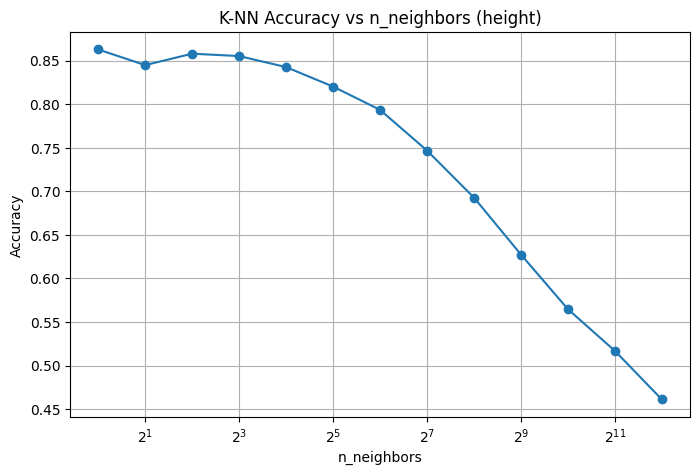
\includegraphics[width=0.8\textwidth]{figures/knn_accuracy.png}
\caption{Accuracy of K-NN classifier on testing data.}
\label{fig:knn_accuracy}
\end{figure}

The accuracy of the K-NN classifier is heavily dependent on the number of neighbours (k) used in the algorithm. Figure \ref{fig:knn_accuracy} shows the accuracy of the K-NN classifier reaches a maximum at 1 neighbour, and then decreases as the number of neighbours increases. This could be related to the high dimensionality of the data.
\\
The K-NN classifier is particularily sensitive to the curse of dimensionality; as the number of dimensions increases, point within the hyperspace are more likely to be equidistant from each other. This means that the K-NN algorithm is less able to distinguish between points, and hence the accuracy of the K-NN classifier decreases. This is a common problem with high dimensional data, and is one of the reasons why dimensionality reduction techniques such as PCA are used.
\\

We can confirm this by looking at the accuracy of the K-NN classifier on the PCA-reduced data. 

% Insert figure of K-NN accuracy on PCA-reduced data here
\begin{figure}[h!]
\centering
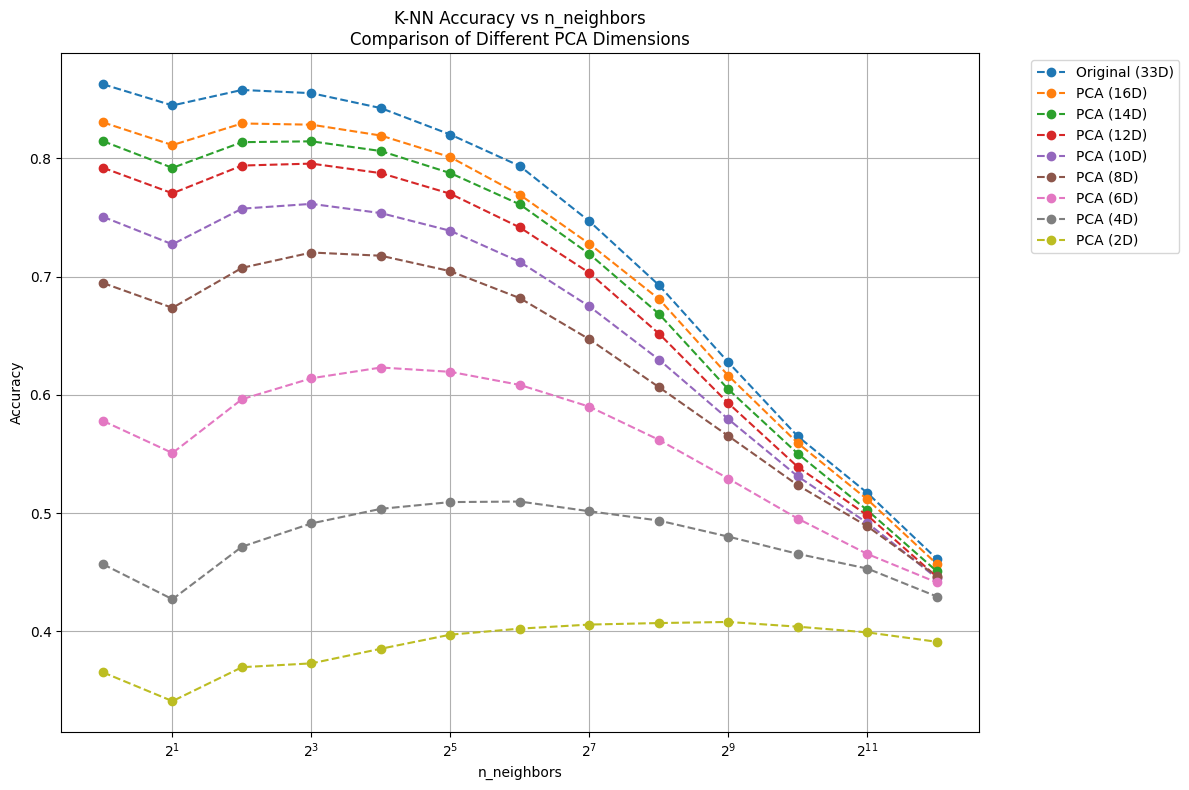
\includegraphics[width=0.9\textwidth]{figures/knn_accuracy_pca.png}
\caption{Accuracy of K-NN classifier on PCA-reduced data.}
\label{fig:knn_accuracy_pca}
\end{figure}


The accuracy of the K-NN classifier on the PCA-reduced data is shown in Figure \ref{fig:knn_accuracy_pca}. As we can see, despite the dimensionality reduction, the accuracy of the K-NN classifier is still highest at 1 neighbour, and then decreases as the number of neighbours increases. This suggests that the decrease in accuracy as neighbours increase is not solely due to the high dimensionality of the data, but also due to the nature of the K-NN algorithm on this particular dataset. This idea is supported by the fact that the curve for each PCA-reduced data (16 to 2 dimensions) is similar to the curve for the original data. 
\\
Additionally, the accuracy of the K-NN classifier decreases as the number of dimensions decreases. If the curse of dimensionality was a significant problem for this dataset, we would expect the accuracy to increase. This suggests that the curse of dimensionality is not a significant problem for this dataset, and that decreasing the number dimensions is not beneficial to the model, as it loses too much information.

\textbf{5.1.1 Computational time after dimensionality reduction}
\\
The computational time of the K-NN classifier is also significantly reduced after dimensionality reduction. The computational time of the K-NN classifier is largest

\vspace{20pt}

\textbf{5.2 K-Fold Cross-validation}

\textbf{6. Random Forest}

\textbf{7. Deep Neural Networks}

\end{document}
